\chapter{Implementación}
\label{chapter:implementation}

El siguiente conjunto de secciones describen la implementación del método
propuesto según las explicaciones presentadas en el Capítulo
\ref{chapter:proposed-method}. La implementación propuesta utiliza el software
de simulación mostrado en \cite{Renz2013}
(\url{https://aibirds.org/other-events/level-generation-competition/basic-instructions.html}),
el cual está programado en Unity, con código fuente en
lenguaje C\#. 

\section{Codificando los diccionarios de piezas}
\label{section:piece_dictionary}

Para poder integrar el listado de piezas al
sistema de generación se decidió la manera en la que se establecerían las
diferentes piezas, como las mostradas en la Figura \ref{figure:game-basic-blocks}
del Capítulo \ref{chapter:proposed-method}, para esto se tomaron en cuenta
varias posibilidades, la primera, cómo se explica en la sección
\ref{subsection:objectorientedidea} se buscaba ordenar las diferentes piezas
cómo diccionarios que contuvieran una o más referencias a las piezas que
integraban cada entrada del diccionario, para esto las primeras 11 posiciones
eran elementos individuales, uno para cada pieza cómo el mostrado en el código
\ref{code:dic_individual_piece}, en el código se aprecia la manera en la que se
designaba una pieza del juego, para poder trabajar de manera dinámica y
agregar más compuestos. Según fuese necesario se utilizaban dos diccionarios
extra, estos contenían los datos de los tipos de materiales y la
información de los tamaños de las piezas, de esta manera en caso de tener más de
una pieza en algún punto del diccionario era posible modificar el valor de
offset de cada una de las piezas calculando la distancia del punto central de
cada pieza al centro de todo el conjunto.

\begin{listing}[t]
  \begin{minted}[frame=lines, framesep=2mm,baselinestretch=1.2,fontsize=\footnotesize,linenos]{python}
    BLOCKS = {
      0: [
          {'type': BLOCK_TYPE['Circle'],
          'material': BLOCK_MATERIAL['wood'],
          'offset': [0, 0, 0] # x, y, z - Calculated from the center of the figure
          }]
    }

    BLOCK_TYPE = {
    'Circle': {'height': 72, 'lenght': 72},
    'RectTiny': {'height': 22, 'lenght': 42},
    'RectSmall': {'height': 22, 'lenght': 42},
    'RectBig': {'height': 22, 'lenght': 42},
    'RectMedium': {'height': 22, 'lenght': 42},
    'RectFat': {'height': 42, 'lenght': 82},
    'SquareTiny': {'height': 22, 'lenght': 22},
    'SquareSmall': {'height': 42, 'lenght': 42},
    'Triangle': {'height': 72, 'lenght': 72},
    'TriangleHole': {'height': 82, 'lenght': 82},
    'SquareHole': {'height': 82, 'lenght': 82}
    }

    BLOCK_MATERIAL = {
        'wood': 0,
        'stone': 1,
        'ice': 2
    }
  \end{minted}
  \caption{Ejemplo de diccionario con un solo elemento}
  \label{code:dic_individual_piece}
\end{listing}

De esta manera, era más sencillo crear compuestos,
sin embargo, la desventaja de utilizar este método era que no se podían
realizar modificaciones a las restricciones de las piezas, por ejempl, para el caso de
querer evitar que un conjunto de piezas con determinados materiales no sean
generados.

En luz de esta información se optó por utilizar el método orientado a objetos
mencionado en la sección \ref{subsection:classorientedidea}, el código
\ref{code:dic_individual_piece_class} muestra la nueva estructura utilizada según el
diagrama de clases presentado en la Figura \ref{figure:pieces-class-diagram},
una clase base con las operaciones y
propiedades necesarias funcionaría cómo una clase base para las clases
de piezas particulares, de esta manera los individuos se representan cómo un
conjunto de referencias a las clases que deben de ser generadas para la
composición de niveles, sin embargo, está manera de representar a los individuos
no contempla las restricciones que pueden ser definidas para la combinación de
piezas-materiales, debido a esto se optó por generar una lista global que
mantuviera un récord de las restricciones aplicadas en el sistema, y al momento
de generar cada re-instanciacion de clase para los individuos está información se
pasará a las clases según fuese requerido, en el código se presenta una variable
con el nombre \textit{mat}, está variable tomará una lista de 3 valores que
define si alguno o algunos de los materiales no puede ser utilizado al momento
de asignar las clases a los individuos, al momento de encontrar una pieza que de
la coincidencia no puede ser utilizada con ningún material se eliminarán los
datos de la pieza generada y se pedirá al sistema genere otra de manera aleatoria.

\begin{listing}[ht]
  \begin{minted}[frame=lines,framesep=2mm,baselinestretch=1.2,fontsize=\footnotesize,linenos]{python}
    class Circle(Piece):
      def __init__(self, mat, x=0, y=0, r=0):
          self.Name = "Circle"
          self.Height = 75
          self.Width = 75
          Piece.__init__(self, x, y, r, mat)
          self.update_values()
  \end{minted}
  \caption{Ejemplo de estructura de las clases hija que heredan de la principal}
  \label{code:dic_individual_piece_class}
\end{listing}

\section{Creación de compuestos}
\label{section:composite_creation}

Una vez definidas las clases que controlarán la información de las
piezas en el algoritmo se procede a definir la manera en la que se entregarán y
controlarán los diferentes compuestos de piezas, para términos más simples los
compuestos son grupos de una o más piezas y se mostrarán a manera de diccionario
de listas cómo se muestra en el código \ref{code:dic_composites}, de esta manera
cada entrada en el diccionario tiene por nombre o apuntador el valor posición
según se fueron agregando al diccionario, mientras que el contenido es una lista
con tuplas donde se estipula la información pertinente de cada pieza en el
compuesto. Un ejemplo claro es el elemento en la posición \textit{9}, el cual
cuenta con 3 piezas que muestran los valores de offset medida desde el centro
del compuesto, visto gráficamente en el juego, está lista se utiliza para
mantener un control de los compuestos que se pueden ir agregando durante la
ejecución del algoritmo, de tal manera que las clases derivadas de
\textit{Composite} harán referencia a una o más piezas según la lista que se
haya proporcionado al crear el compuesto.

\begin{listing}[ht]
  \begin{minted}[frame=lines,framesep=2mm,baselinestretch=1.2,fontsize=\footnotesize,linenos]{python}
    Composites = {
      0: [("RectTiny", 0, 0, 0, "wood")],
      1: [("RectSmall", 0, 0, 0, "wood")],
      2: [("RectMedium", 0, 0, 0, "wood")],
      3: [("RectBig", 0, 0, 0, "wood")],
      4: [("RectFat", 0, 0, 0, "wood")],
      5: [("SquareSmall", 0, 0, 0, "wood")],
      6: [("SquareHole", 0, 0, 0, "wood")],
      7: [("Circle", 0, 0, 0, "wood")],
      8: [("TriangleHole", 0, 0, 0, "wood")],
      9: [("RectBig", 100, 5, -27, "wood"), ("RectBig", -100, 5, 27, "wood"), ...
            ...("RectSmall", 0, 0, 90, "wood")]
    } 
  \end{minted}
  \caption{Diccionario con los compuestos existentes}
  \label{code:dic_composites}
\end{listing}

\section{Definición de clase auxiliar de individuo}
\label{section:definition_of_clases}

Mediante el uso de la clase \textit{Composite}, se tiene un mejor control de los genes
que conformarán cada individuo de la población. El siguiente paso es el de 
programar la clase que llevará el control de los cromosomas de un individuo, 
siendo los cromosomas los compuestos asignados a cada individuo, de tal manera que un individuo
dentro de la información de cromosomas hará referencia a otra lista de
compuestos, la manera en la que un \textit{Individuo} relaciona los compuestos es
mediante el uso de la línea de código:

\begin{minted}{python}
  chromosome_objects = [Composite(Composites[composite]) for composite in self.chromosome]
\end{minted}

Mediante esta línea de código, se crea una lista en donde
cada elemento será una instancia de un compuesto asignado al individuo, de está
manera si se requiere modificar la posición o materiales de un compuesto
particular en el individuo es posible hacerlo desde la clase de
\textit{Individuo}, de igual manera está clase tiene otras funciones 
como se muestra en el diagrama de clase de la Figura
\ref{figure:individual-class-diagram}, por ejemplo, realizar los cálculos de fitness y generar
las listas de piezas que serán utilizadas para generar los archivos de salida
para las simulaciones de los niveles generados.

\section{Generación de individuos}
\label{section:ind_generation}

Una vez definida la manera de controlar las clases el paso siguiente es el de
comenzar con la generación de ls individuos de la población, para poder lograr
esto se creó una línea de código en la cual los puntos necesarios para la
generación de los individuos se entregan totalmente, mediante la siguiente 
línea de código: 

\begin{minted}{python}
  pop = [Individual(chromosome = get_random_chrom(ind_pieces), ..
    ..másk = create_new_másk(ind_pieces)) for i in range(population)]
\end{minted}

Mediante el uso de esta línea de código se le indica al sistema que se requiere
una lista que representará a los individuos de la población, cada elemento de
está lista será una instancia independiente de la clase \textit{Individual},
para generar está instancia de clase es requerido dos valores siendo estos
primero una lista de valores numéricos que representan cuales piezas se
asignaran a los individuos, para generar está lista se utiliza una función cómo
se muestra en el código \ref{code:get_random_chrom}, el segundo dato requerido
es una segunda lista que denota una máscara mediante la cual las piezas
asignadas serán acomodadas al momento de generar los archivos de simulación,
finalmente, la última sección del código - \textit{for i in range(population)} -
denota que el proceso se deberá de repetir una cierta cantidad de veces, es
decir que pada cada individuo se generara una instancia con valores diferentes a
los anteriores, la cantidad de vences que se deberá de repetir depende de la
cantidad de individuos con los que se quiere estar trabajando en el algoritmo en
el caso de las pruebas realizadas se utilizó un total de 10 individuos lo que
significa que la lista \textit{pop} generada consta de 10 instancias diferentes
de la clase \textit{Individual}. 

Para la generación de la lista de piezas o cromosomas asignados a un individuo
mostrada en la parte (1) del código en \ref{code:get_random_chrom}, aquí el
valor que se recibe denota la cantidad de piezas o compuestos que se deberán de
asignar en la lista del individuo, para asignar estos valores primero se
obtiene un número aleatorio que va desde \textit{0} hasta la cantidad de piezas o
compuestos presentes en la lista, menos la unidad, para evitar errores de
posicionamiento de lista. Posteriormente se revisa si la pieza seleccionada
puede ser utilizada al menos en una combinación dentro de la generación, en caso
de que no pueda ser utilizada se obtiene otra y de igual manera se revisa, en
caso de poder ser utilizada, se agrega a la lista y avanza un contador para saber
cuando se llegue al límite de piezas posibles. Finalmente se entrega la
lista de piezas para la generación de la instancia de clase. Para la generación
de la máscara de acomodo de piezas, se utiliza la sección de código mostrada en
la parte (2). En esta parte se revisa la cantidad de
compuestos que se pueden utilizar, cómo en la parte anterior, este valor se
utiliza posteriormente para generar una lista aleatoria, la lista que se genera
tiene un total de 7 posiciones que denotan las 7 divisiones que se realizan en el
área de un nivel para el acomodo de las piezas. Mediante el uso del valor de
piezas en cada individuo se realiza una aleatorización de números desde
\textit{0} hasta la cantidad máxima de piezas, una vez que se obtienen estos valores
aleatorios se revisa si la suma de estos da la cantidad de piezas en el
individuo, en caso de que no sea así, se repite el proceso, en caso de que si se
cumpla entonces la lista se regresa para la creación del individuo.

\begin{listing}[ht]
  \begin{minted}[frame=lines, framesep=2mm, baselinestretch=1.2, fontsize=\footnotesize, linenos]{python}
 (1)  def get_random_chrom(sl):
        asl = 0
        chrom = []
        while asl < sl:
            prop = random.randint(0, len(Composites)-1)
            if clases[Composites[prop][0][0]].Valid == True:
                chrom.append(prop)
                asl += 1
        #random.randint(0,len(Composites)-1) for p in range(ind_pieces)
        return chrom

 (2)  def create_new_másk(pieces):
        div_list =[]
        while True:
            div_list = [random.randint(0, pieces-1) for col in range(7)]
            if sum(div_list) == pieces:
                break
          
        return div_list
  \end{minted}
  \caption{Código de asignación de cromosomas(piezas)[1] y código para generar máscaras [2]}
  \label{code:get_random_chrom}
\end{listing}

Una vez que se ha logrado crear la lista de individuos se procede a inicializar
el algoritmo evolutivo, este algoritmo se ejecutará una determinada cantidad de
veces, el pseudocódigo se enlista a continuación en el código
\ref{code:algorithm_pseudocode}, este pseudocódigo engloba los aspectos
principales del sistema de generación de niveles, el código se explica más a
detalle en las secciones siguientes.

\begin{listing}[ht]
  \scalebox{.8}{\noindent%
\begin{Heardlisting}{%
   \begin{tabular}{r}% 
      Integrar miembros "elite" (1-4)\\ \\  \\  \\  \\
      Simular individuos (6)\\  \\
      Calcular fitness (8-9)\\  \\  \\
      Obtener padres de la generacion (10)\\  \\
      Realizar crossover (12)\\ \\
      Seleccionar elite (14-15)\\ \\
   \end{tabular}
}
if elite not null
   for member in elite
      population <- member
      trim population

execute process (game)

for individual in population
   individual.getfitness

parents <- selector_operator(population, required)

crossover_operation(population, parents)

population.order('fitness')
elite.add(population[1])
\end{Heardlisting}}
  \caption{Pseudo-código del algoritmo genético}
  \label{code:algorithm_pseudocode}
\end{listing}

\subsection{Integración de miembros elite}
\label{subsection:elite_member_integration}

Está parte se encarga de iniciar los bucles de generación, la función principal
de este bloque de código es la revisar la lista auxiliar de miembros de elite
que existe en memoria, en caso de tener elementos en la lista estos se integran
a la lista de la población integrándose al inicio de la misma, una vez agregados
todos los miembros la lista de la población se corta hasta el número máximo de
miembros permitidos en las generaciones, este valor se asigna cómo un valor de
entrada al inicio del archivo que contiene el código.

Una vez terminada esta acción se procede a denotar la cantidad de padres que
serán necesarios para generar los hijos de las generaciones futuras, esto se
hace mediante el cálculo:
\begin{minted}{python}
  many = len(pop) * per_cross
\end{minted}
En donde \textit{pop} representa la lista de miembros de la población,
\textit{per\_cross} representa un valor entre \textit{0\.0} y \textit{1\.0}, este
valor representa que tanto porcentaje de la población realizará cruces,
de esta manera la variable \textit{many} representa la cantidad de individuos
que se deberán utilizar para cumplir el porcentaje de cruce, debido a que el
valor de \textit{per\_cross} puede generar un valor flotante se tiene una parte
de código en donde si el total de individuos que realizarán cruces es un número
impar entonces el valor que se deberá de utilizar será el numero par redondeado
hacia abajo, es decir, si de 10 individuos en la población se quiere que un
total de individuos cercano al \textit{50\%} realicen un cruce entonces el valor
resultante para la variable \textit{many} sería de 5, en este caso lo que se
hace es restar 1 al resultado y después se redondea hacia abajo, lo cual haría
que el número de padres requeridos para los cruces sea de 4.

Una vez que se tiene el valor de los padres requeridos para los cruces de la
generación se procede a crear los archivos auxiliares de los individuos de la
población, los archivos generados son en formato \textit{XML}, la información
que contienen estos archivos es la posición, tipo y material de ls piezas que
serán utilizadas en el nivel, además de esto también contiene la información de
la cantidad y tipo de aves así cómo de los enemigos que serán colocados, estos
archivos son almacenados en un folder en donde el software de simulación se
encarga de obtenerlos y entregar los resultados después de la simulación.

Una vez que los archivos de simulación han sido generados el algoritmo manda un
comando que manda la ejecución del software de simulación, el software en
particular cuenta con una ventana gráfica en la que se puede apreciar los niveles
que se generaron o evolucionaron en caso de estar simulando archivos de una
generación después de la primera, de igual manera el software genera un archivo
en formato \textit{XML}, similar al que se genera antes de la simulación, la
diferencia entre ambos archivos es que el entregado después de la
simulación entrega los datos de posición de el último estado registrado del nivel,
además de que se puede solicitar que entregue el valor de la aceleración de la
misma. El valor de aceleración es tomado en cuenta desde el punto en el que la
pieza comienza su descenso, en caso de que una pieza sea destruida durante el
proceso de simulación ninguno de los datos de esa pieza son grabados en los
archivos, la manera de llevar control de las piezas que entran y las que salen
es mediante el uso de un número de lista asignado al momento de generar los
archivos de simulación de la sección anterior.

Posterior a la simulación los archivos entregados son revisados y en base a la
información de las piezas se calcula el \textit{Fitness} de las mismas,
posteriormente a esto se procede a ordenar la lista, y realizar las operaciones
de selección, cruce y mutación los cuales se explican en la sección siguiente.

\subsection{Operador de selección}
\label{subsection:sel_operator}

El proceso de selección se definió de dos maneras, la primera es
mediante el uso de una ruleta, en está ruleta los valores que
se toman en cuenta es el fitness de cada individuo, mientras más alto sea el
fitness mayor será la probabilidad de ser seleccionado para el cruce en la
siguiente sección.

El segundo método utilizado es la selección mediante torneo, en este tipo de
selección lo que se realiza es que los individuos se seleccionan en pares de
manera aleatoria, entre cada par se realiza un cálculo de cual tiene el mejor
fitness y ese individuo es seleccionado cómo padre para la generación.

\subsection{Operador de cruce}
\label{subsection:crossover_operator}

Para los operadores de cruce se tienen codificados dos tipos, cruce de un punto
y cruce de dos puntos, este operador de cruce se realiza no solo en los
individuos de la población sino también en las máscaras que tienen los mismos
individuos, esto es para aumentar un grado más el nivel de diversidad que se
puede tener en los individuos generados, la idea en este caso es lograr que
existan casos en donde la máscara sea muy chica y varias piezas de los
individuos no sean mostradas y el caso contrario permitirá que un individuo
pueda o no quedar con el mismo caso y puede que se dé el caso en donde alguno de
ambos elementos logren obtener un mejor nivel de fitness en la generación.

Un ejemplo de estos dos tipos de cruce se puede apreciar en la Figura
\ref{figure:crossover} en donde dos individuos realizan un cruce con sus
máscaras y las máscaras generadas para los hijos resultan con diferente cantidad
de piezas.

La manera en cómo se aplican estos tipos de operador es:
\begin{enumerate}
  \item Definir un punto de corte igual para los dos individuos en cualquier
  posición de la lista de genotipos.
  \item Separar las dos partes cortadas de ambos individuos de tal manera que se
  tenga la parte de inicio (del inicio hasta el corte) y la parte final (desde
  el corte hasta el final) de cada individuo.
  \item Para crear al primer hijo tomar la parte inicial del primer individuo y
  unirla con la parte final del segundo individuo
  \item Para el segundo hijo tomar la parte inicial del segundo individuo y
  unirla con la parte final del primer individuo.
\end{enumerate}
De está manera los hijos se pueden comprender de la siguiente manera:
\begin{minted}{python}
  padre1 = padre[1, punto_corte]
  padre2 = padre[punto_corte, fin]

  madre1 = madre[1, punto_corte]
  madre2 = madre[punto_corte, fin]

  hijo1 = padre1 + madre2
  hijo2 = madre1 + padre2
\end{minted}

Para el caso del cruce de dos puntos, en vez
de dividir el genotipo de un individuo en dos partes, se divide en tres y al
momento de realizar la combinación se toma la primer parte del primer individuo,
después la parte de enmedio del segundo individuo y finalmente la parte final
del primero, de tal forma que solo la parte central de ambos individuos se
cambia.

\begin{figure}
  \centering
  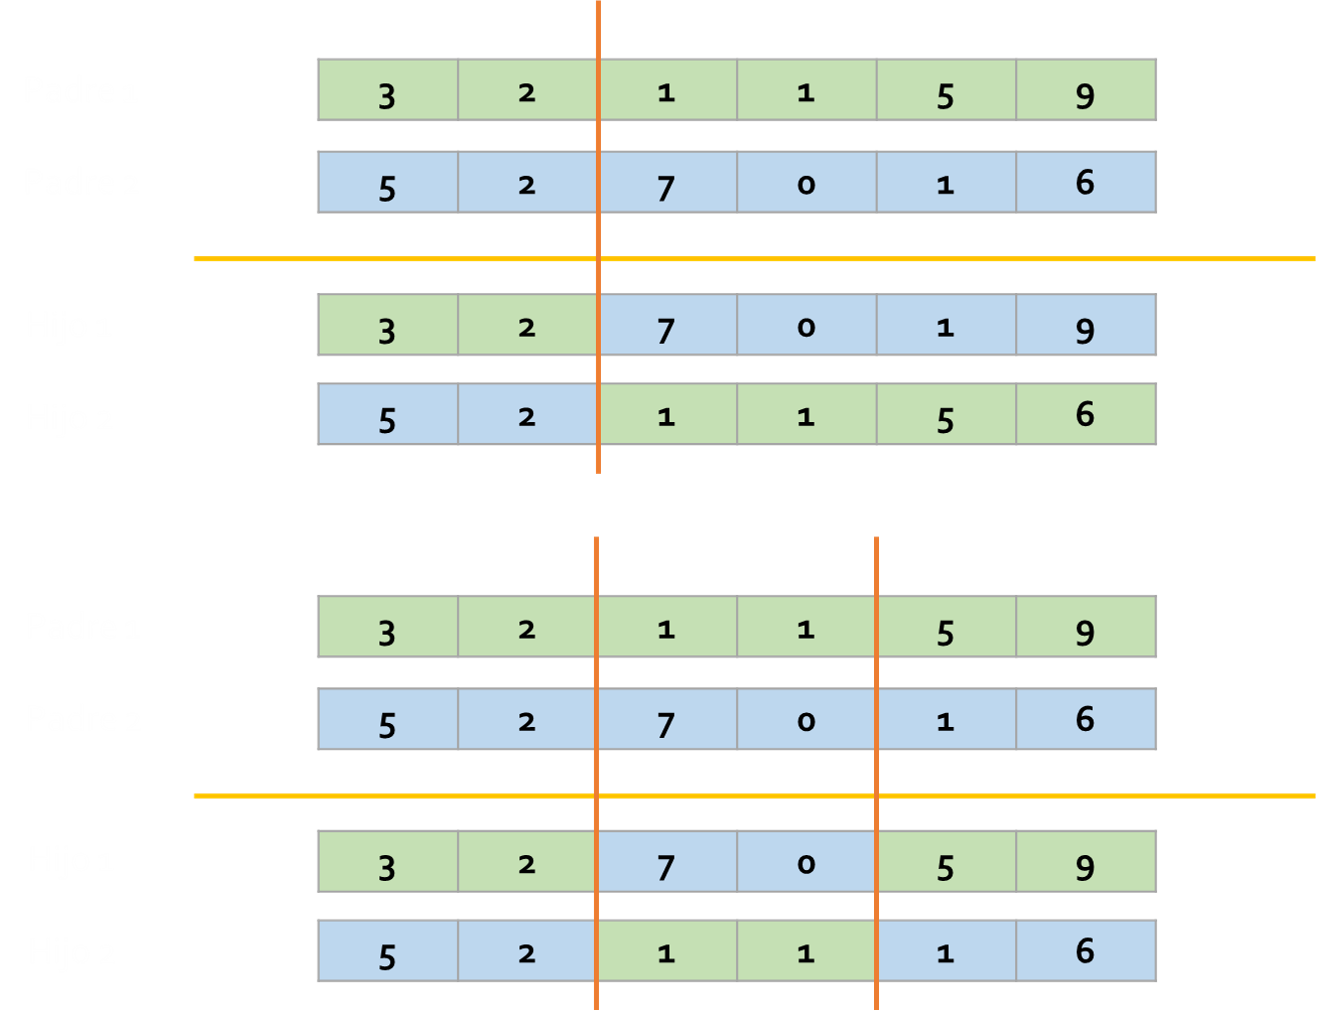
\includegraphics[width=0.8\textwidth]{img/crossover_es.png}
  \caption{Cruce de un punto (arriba) y cruce a dos puntos (abajo) aplicada a la máscara de individuos}
  \label{figure:crossover}
\end{figure}

\subsection{Operador de mutación}
\label{subsection:mutation_operator}

La mutación de los individuos de la población ocurre solo al momento de hacer el
cruce de los mismos, es decir solo a los elementos nuevos se les aplica el
operador de mutación, este operador puede modificar los siguientes elementos de
un individuo:

\begin{enumerate}
  \item La cantidad de piezas que conforman al individuo.
  \item El material del cual están formados los elementos.
  \item El tipo de elemento que conforma a un individuo, es decir, modificar el
  valor del compuesto que forma parte del individuo.
  \item La posición individual (\textit{x} o \textit{y}) de los compuestos.
\end{enumerate}

El operador de mutación se describe cómo sigue,
primero al momento de generar al nuevo individuo se realiza un cálculo de
porcentaje en donde se decide si tendrá o no mutación, dependiendo del porcentaje
de mutación que se haya asignado al inicio del algoritmo, posteriormente en caso
de que el valor de porcentaje quede dentro del rango, se toma para las
operaciones siguientes:

Para mutar la cantidad de compuestos en un individuo primero se realiza una
selección aleatoria entre las opciones de agregar o quitar compuestos,
posteriormente en caso de requerir agregar más se realiza una selección
aleatoria de entre la cantidad de compuestos creados, estos mismos se integran
al final de la lista de compuestos del individuo. Para eliminar elementos de la
lista se realiza una corrida por todos los elementos y en cada uno se realiza
una probabilidad de \textit{50\%} de sea borrado de la lista, un ejemplo de este
proceso se muestra en la Figura \ref{figure:mutate_add_remove} en donde se
presenta una tabla que denota las posiciones de los compuestos en base a la
máscara, en este ejemplo se realizó una corrida para remover elementos (color
rojo) y una segunda para agregar nuevos compuestos (color verde).

\begin{figure}
  \centering
  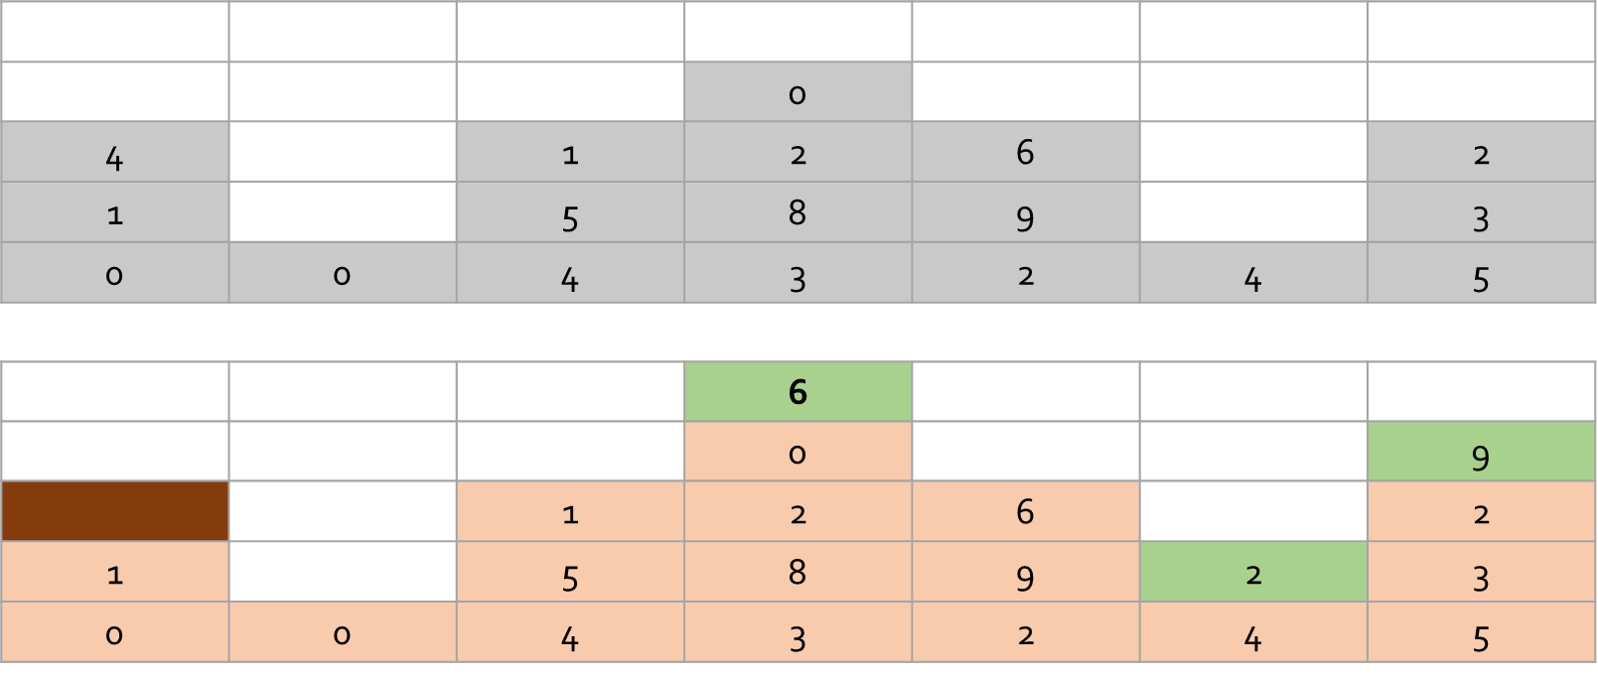
\includegraphics[width=0.85\textwidth]{img/mutation_add_remove.png}
  \caption{Ejemplo del operador de mutación enfocado a remover y agregar compuestos}
  \label{figure:mutate_add_remove}
\end{figure}

La segunda mutación se encarga de modificar el material del que están
conformados los compuestos del individuo, primero se selecciona aleatoriamente 
cuales compuestos serán modificados sin
repetir valores, posteriormente se modifica de manera aleatoria el valor que
define el tipo de material del que se conforma, para esto se toma en cuenta que
\textit{0} representa material de madera, \textit{1} representa material de
hielo y finalmente \textit{2} representa el material de piedra, debido a que el
juego solo acepta está lista de compuestos no es posible asignar valores
diferentes a estos.

En la Figura \ref{figure:mutate_material} se muestra un ejemplo de la manera en
cómo opera la mutación del tipo de compuesto, en este ejemplo se muestra el
genotipo y fenotipo de un individuo, el genotipo muestra los colores naranja,
azul y gris para denotar los materiales de madera, hielo y piedra
respectivamente, en este caso la mutación cambia el material de 5 elementos del
genotipo de madera a hielo, esto se refleja del lado derecho en donde se muestra
la vista actualizada del individuo después de la mutación.

Debido a que los compuestos generados pueden contener diferentes cantidades de
elementos en estos casos se cambia el material equitativamente a todos elementos
del compuesto, de esta manera se evita tener que realizar un recorrido por todo
el compuesto y mutar el material de cada uno.

\begin{figure}
  \centering
  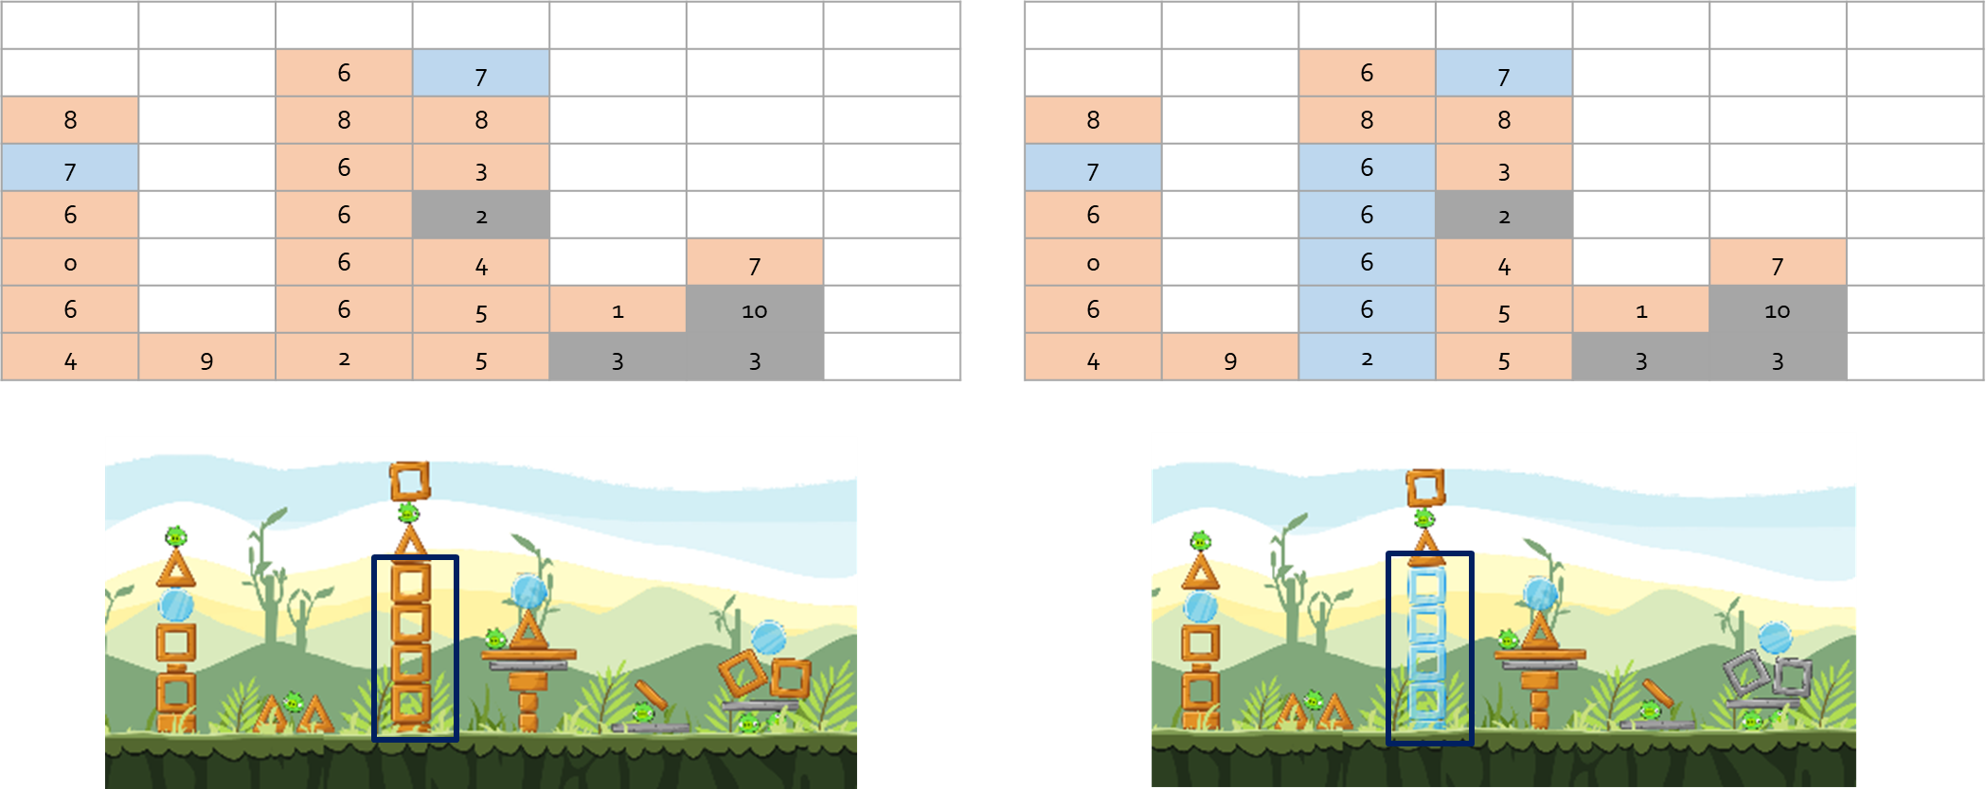
\includegraphics[width=0.95\textwidth]{img/mutation_material.png}
  \caption{Ejemplo del operador de mutación enfocado a cambiar el material de los compuestos, pre-mutación (izquierda) y post-mutación (derecha)}
  \label{figure:mutate_material}
\end{figure}

La tercera mutación se encarga de cambiar el compuesto que representa una
posición del genotipo del individuo, este trabaja de una manera similar al
anterior en el sentido de que primero se selecciona a los individuos a mutar,
posteriormente a la selección se realiza una segunda selección aleatoria entre
las posiciones del genotipo del individuo, aquellos compuestos seleccionados son
cambiados por otro de la lista existente, para esto se realiza una selección de
un valor aleatorio que va desde \textit{0} hasta la cantidad de compuestos
existentes, por ejemplo, suponiendo que se tiene solo la cantidad base de piezas
en el algoritmo entonces la selección será un valor aleatorio desde \textit{0}
hasta \textit{10}.

La Figura \ref{figure:mutate_composite} nos muestra un ejemplo de cómo es que
actúa la mutación de tipo de compuesto, en el ejemplo mostrado se tiene el
genotipo de un individuo combinado con su respectiva máscara así cómo su
fenotipo respectivo (lado izquierda) al ser representado en la pantalla del
juego, en el lado derecho de la misma imagen se aprecia la modificación de
compuestos realizada al genotipo base (marcado en amarillo), la modificación de
compuestos en los individuos puede traer la consecuencia de que los niveles
generados sean inestables cómo en este ejemplo, esto a su vez puede permitir
identificar máscaras de los individuos que logran mantener la estabilidad de las
estructuras permitiendo así mejorar el algoritmo.

\begin{figure}
  \centering
  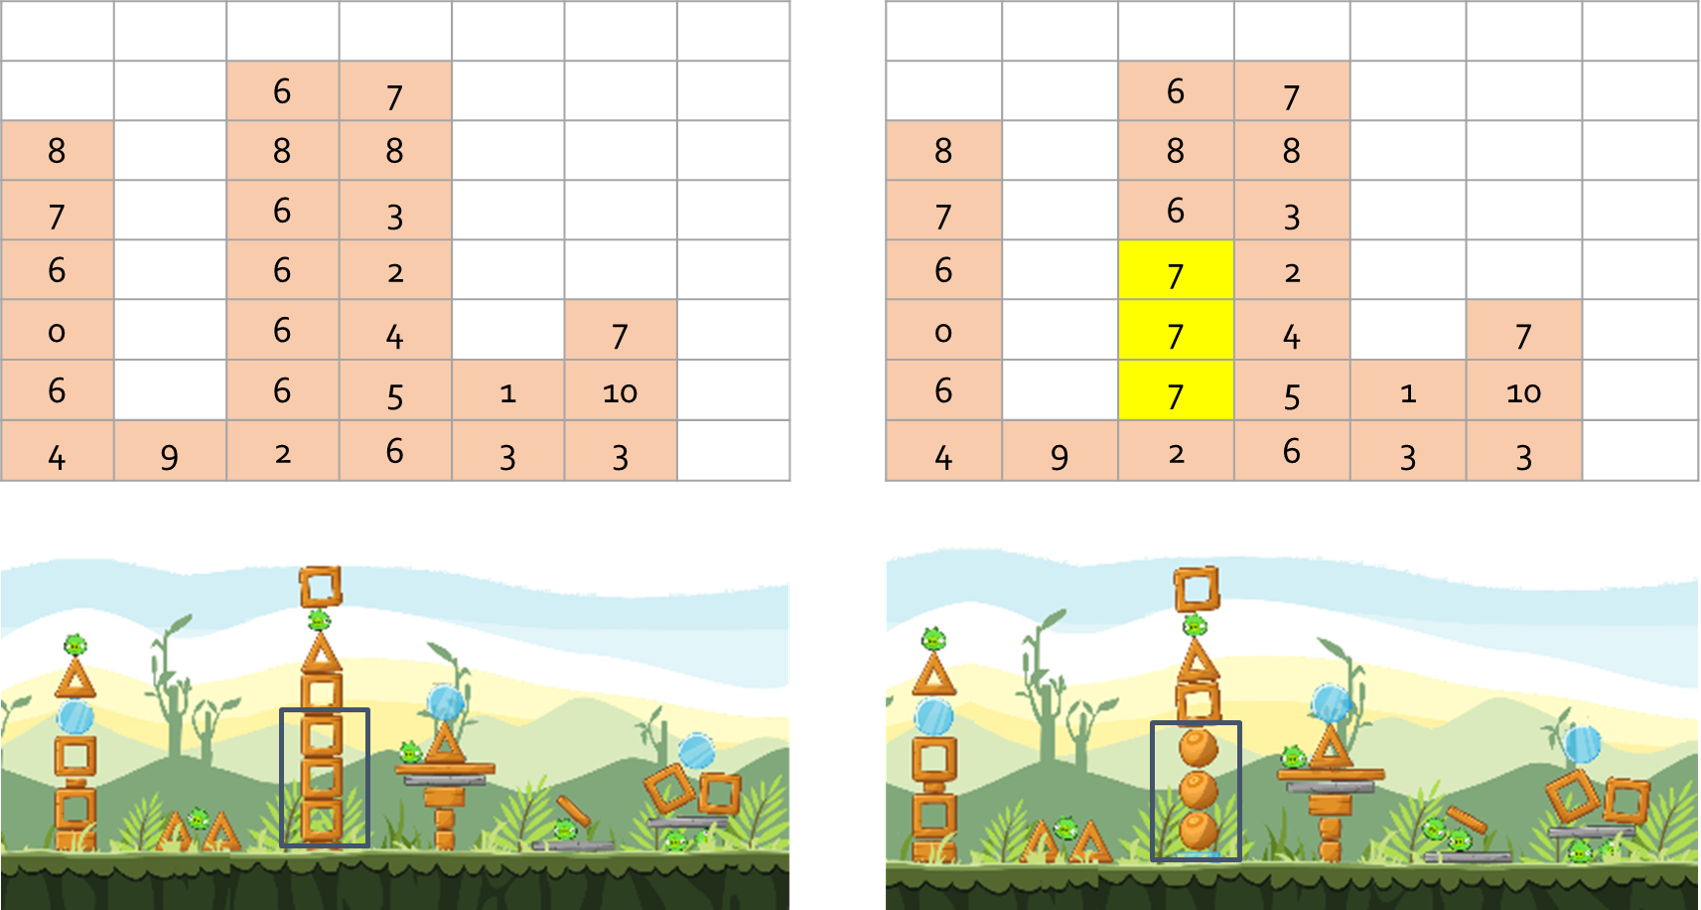
\includegraphics[width=0.9\textwidth]{img/mutation_composite.png}
  \caption{Ejemplo del operador de mutación enfocado a cambiar los compuestos asignados, pre-mutación (izquierda) y post-mutación (derecha)}
  \label{figure:mutate_composite}
\end{figure}

El último tipo de mutación realizada en los individuos es la modificación de las
posiciones \textit{x} y \textit{y} de algunos compuestos dentro del individuo,
la modificación de las posiciones se realiza mediante una selección de valores
aleatorios de una distribución gaussiana dentro de un cierto rango de distancia
para no permitir que los elementos se alejen demasiado de punto central
original.

\subsection{Representacion de individuos}
\label{section:individual_representation}

Una vez que se han agregado nuevos individuos a la población, y que estos
individuos pasaron por su fase de mutación, si es que requerían, se procede a
realizar la combinación de los elementos que conforman al individuo con el fin
de generar los archivos requeridos para la simulación de estos mismos. Cabe
resaltar que está combinación se realiza también en los individuos iniciales
antes de la simulación inicial, debido a que el juego requiere una
representación mediante el uso de archivos en formatos \textit{XML}, se requiere
primero obtener la información de todos los elementos que conforman a un
individuo y posteriormente armar los archivos mediante el uso de estos datos.

\begin{figure}
  \centering
  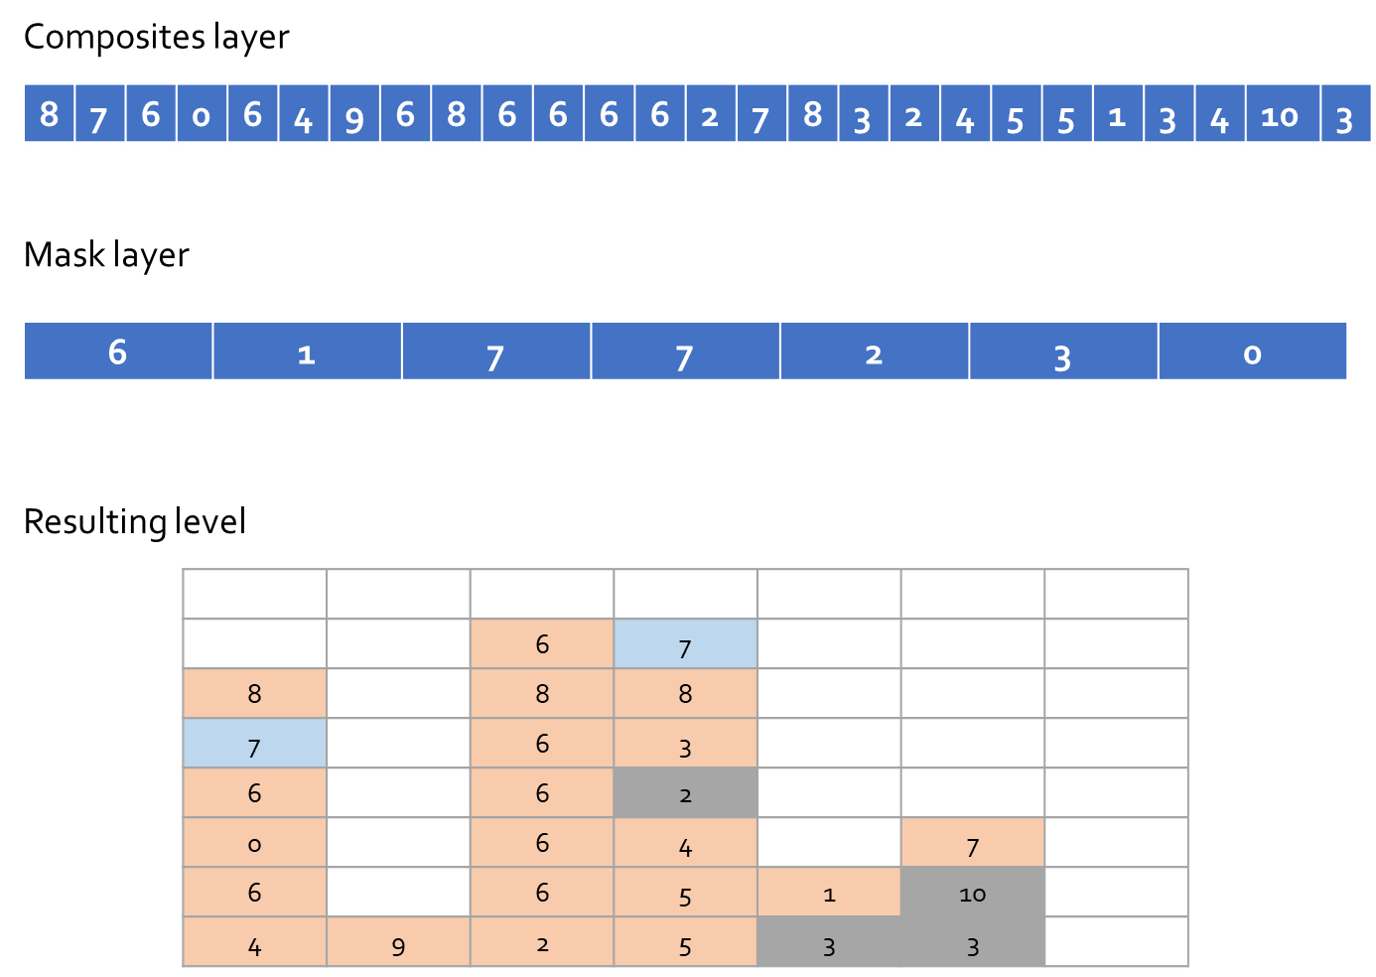
\includegraphics[width=0.9\textwidth]{img/layer12_combine.png}
  \caption{Ejemplo de la combinación de capas de un individuo}
  \label{figure:individual_representation}
\end{figure}

En la Figura \ref{figure:individual_representation} muestra la estructura de los
componentes de un individuo, un individuo es representado por \textit{2} capas
diferentes en forma de lista, la primera es la capa de compuestos, está capa se
muestra la lista de compuestos que representan a un individuo, esta lista puede
variar en tamaño, dependiendo de si durante las operaciones de mutación se le
agregaron o quitaron elementos al individuo, de igual manera cómo se explicó en
el la sección \ref{section:composite_creation}, cada valor de la lista representa
no una pieza del juego sino uno de los compuestos que se crean antes de iniciar
el algoritmo o aquellos que se agregan durante el mismo.

La segunda parte que compone la representación del individuo es la máscara, cómo
se explica en la sección \ref{subsection:ruleofthirds}. La idea detrás del uso de
está máscara, es la de generar estructuras utilizando la lista de compuestos del
individuo, en esta misma sección se presentó una propuesta de crear máscaras en
donde se denotará la forma que se quería que tuviera un individuo particular,
aplicando estás estructuras en los individuos, generaba los resultados esperados,
siendo el caso niveles en donde la distribución de los compuestos crearan formas
diferentes cómo castillos, torres, casas o diferentes figuras. Sin embargo
utilizar este tipo de estructuras no permitía que el algoritmo lograra
evolucionar, sino que simplemente encontraría la mejor combinación de
piezas-máscara en determinado momento, por esto se optó por utilizar la
generación de máscaras que se muestra en la Figura
\ref{figure:individual_representation} y que fue explicado en la sección
\ref{section:ind_generation} la cual únicamente muestra una determinada cantidad
de piezas a asignar en posiciones diferentes del nivel, esto permite tener mejor
diversidad en los individuos creados.

Al momento de combinar ambos componentes del individuo se obtiene un resultado
similar al mostrado en la parte inferior de la imagen en donde los compuestos se
organizan en manera de cola, es decir el primer elemento en la lista será el
primero en ser colocado, una vez que se definen cuales elementos serán colocados
en cada columna, el sistema calcula la altura total de cada compuesto y
comenzando desde la parte inferior coloca un compuesto en el nivel, después
calcula la distancia desde la parte superior del mismo hasta la parte central
del siguiente para colocarlo de tal forma que al comenzar la simulación no
aparezcan en caída libre, sino que aparezcan una pieza sobre otra, de esta manera
se previenen problemas de balance al permitir que las piezas caigan y
reboten en direcciones que provocaran que las estructuras terminen por caer
totalmente, en la misma imagen se aprecian cuadros de diferentes colores, estos
mismos representan el material del cual está construido cada compuesto cómo se
explicó en la sección de mutación anterior.

Finalmente, una vez que se tiene la información anterior definida se procede a
realizar una búsqueda de los lugares en donde aparecerán los enemigos del juego,
se define dónde pueden aparecer estos mediante una función
que revisa los compuestos que existen en el nivel. Cuando un compuesto cumple
con ciertas características se permite que uno de los enemigos pueda ser
colocado en la parte central o superior del mismo, al iniciar este método se
busca aquellos que cumplen esta característica y se ordena en una lista
auxiliar, después de manera pseudo-aleatoria se decide la cantidad de enemigos
que tendrá el nivel, de acuerdo a este valor se seleccionan \textit{x} cantidad
de posiciones para colocar a los enemigos donde \textit{x} es el valor de
enemigos requeridos, una vez se definió en donde estarán colocados estos
enemigos se regresa una lista con las coordenadas \textit{x} y \textit{y} de las
mismas.

Mediante la combinación de los enemigos con el genotipo construido de un
individuo se obtiene el nivel a mostrar en el juego, una representación de esto
se muestra en la Figura \ref{figure:ind_representation_plus_pigs}, en donde al
genotipo armado de acuerdo a los puntos anteriormente mencionados se le agrega el
listado de posiciones de los enemigos. En este caso los enemigos son
representados por un color verde en las posiciones en donde estarán. 
Esto permite tener la estructura de los niveles completa, esta información se
utiliza al momento de generar los archivos de \textit{XML} los cuales en el
software de simulación generarán una vista de los mismos, cómo se muestra en la
esquina inferior derecha de la misma imagen. 

\begin{figure}
  \centering
  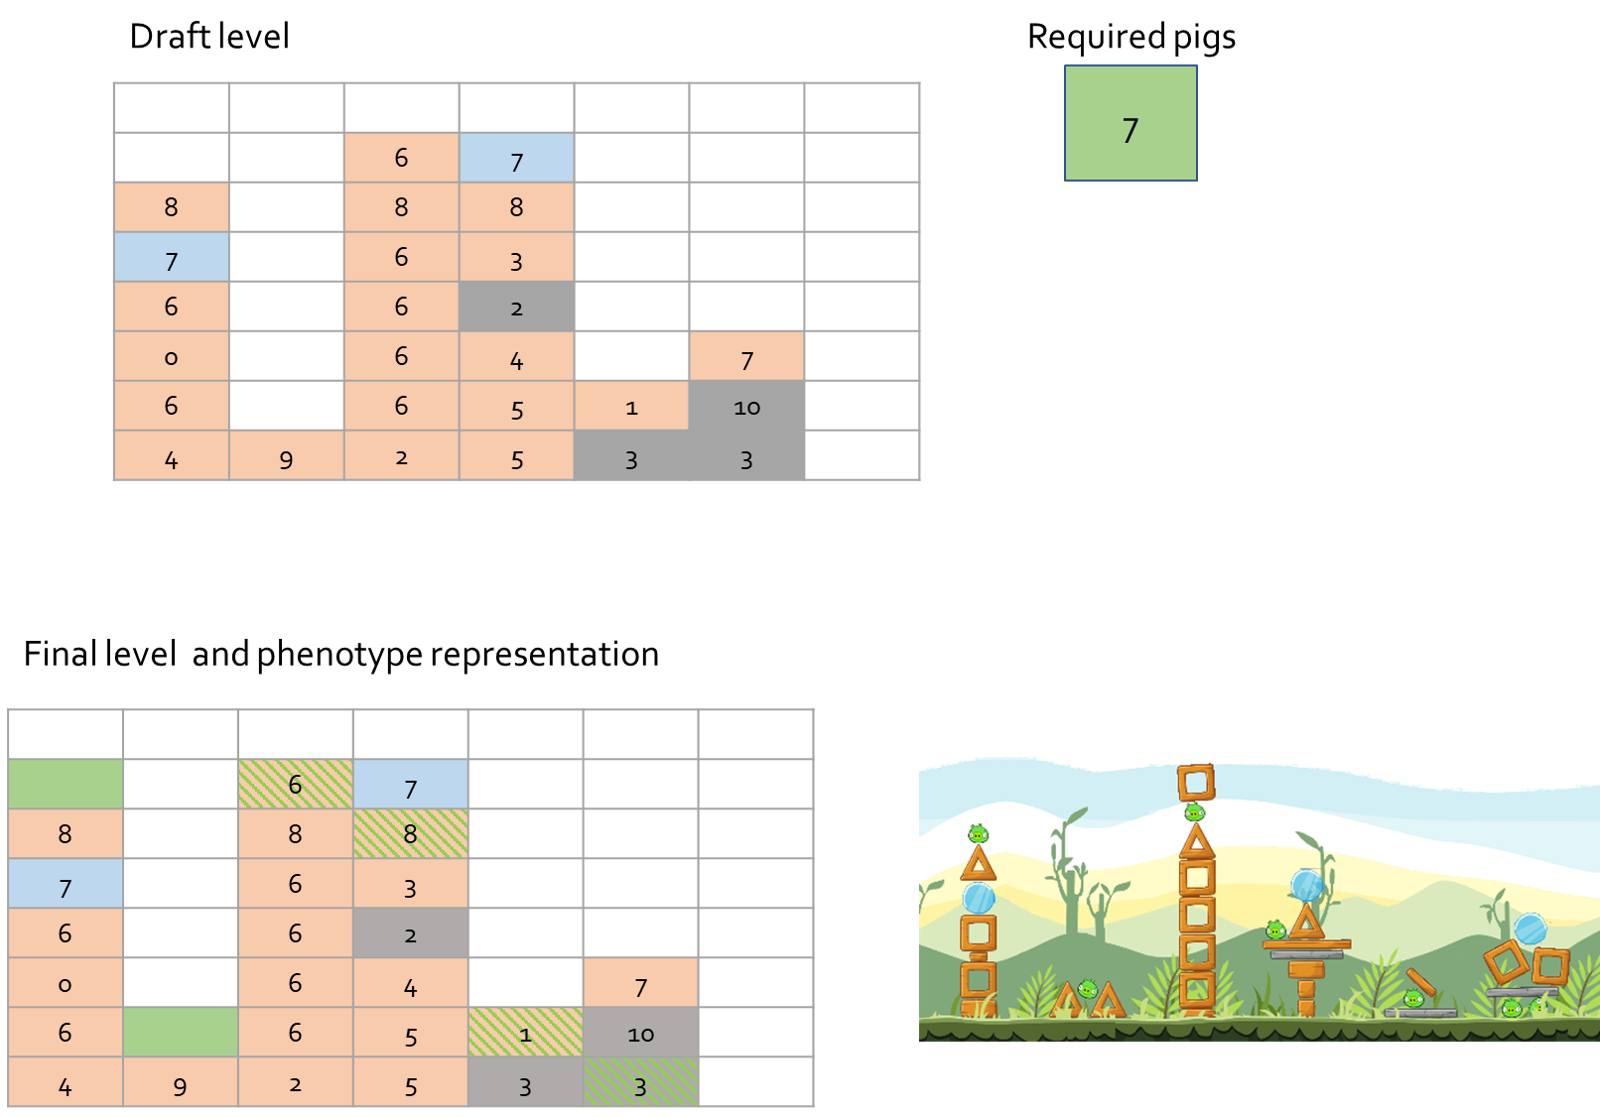
\includegraphics[width=0.9\textwidth]{img/layer123_combine.png}
  \caption{Ejemplo de la combinación de un genotipo armado de la Figura \ref{figure:individual_representation} con la colocación de enemigos}
  \label{figure:ind_representation_plus_pigs}
\end{figure}

\subsection{Cálculo de fitness}
\label{subsection:fitness_calculation}

Cuando los individuos pasan por el proceso de simulación se genera un archivo en
formato \textit{XML} que contiene los resultados de los compuestos que fueron
puestos en los archivos antes de la simulación, con la diferencia de que estos
archivos contienen la información del último estado de los mismos compuestos. Al
terminar dicha simulación, se obtiene un listado de piezas y enemigos con
la información de sus posiciones \textit{x} y \textit{y} así cómo del ángulo con
en el cual quedaron al concluir la simulación, además de esto se entrega la
información de la velocidad promedio del movimiento que tuvieron.

Está información permite conocer las imperfecciones que tuvieron los niveles al
concluir las simulaciones, para mejorar la evaluación obtenida que determina la
aptitud de los individuos se toma en cuenta una evaluación de dos fases, la
primera fase tiene que ver con la estabilidad de los individuos y se evalúa en
base a dos métricas:
\begin{enumerate}
    \item La cantidad de piezas que no son destruidas durante la simulación.
    \item Las posiciones finales de dichas piezas al terminar la simulación.
\end{enumerate}

Para poder realizar el cálculo de las piezas presentes antes y después de la
simulación se utiliza la información de las piezas anteriormente mencionada, sus
posiciones tanto \textit{x} cómo \textit{y} así cómo del angulo de las mismas, a
está información se le agrega un indicador de posición para poder compararlo con
los datos del mismo indicador para las funciones siguientes, está listado de
información se realiza también antes de la simulación con el fin de tener datos
con los cuales comparar, una vez que se tienen los datos se procede a realizar
el proceso de cálculo de fitness, para calcular le diferencia de piezas se
compara la cantidad de elementos en ambas, debido que al momento de caer de
alturas grandes algunos elementos tienden a romperse entonces la cantidad de
elementos después de la simulación podrá ser menor, para obtener el primer valor
se realizará un cálculo para obtener un valor entre \textit{0} y \textit{100}
que define la calificación en forma de porcentaje del total de piezas que se
salvaron en la simulación, es decir, si antes de la simulación se tenía un total
de \textit{10} piezas y al terminar la simulación en el archivo correspondiente
solo existen \textit{5} entonces el individuo tendrá una calificación de
\textit{50\%} debido a que solo la mitad de las piezas no fueron destruidas.

El segundo valor toma se utiliza para definir si los conjuntos que no se
destruyeron se lograron mantener los más estábles posible, esto se calcula
mediante el uso de dos fórmulas mostradas en las formulas
\ref{equation:error_pos} y \ref{equation:error_ang} mediante el uso de estás
formulas se comprueba si las piezas lograron o no mantenerse en sus posiciones
originales. En los casos donde las piezas no se hayan destruido se utilizan
estás fórmulas para revisar si las posiciones y ángulos de inicio y final de la
simulación son los mismos, en caso de que así sea, no se modifica el fitness
obtenido previamente, en caso contrario se obtiene una
penalización al fitness, equivalente a una tercera parte del valor de porcentaje
por una pieza si se movió de posición y otra tercera parte, si su ángulo cambió.

\begin{equation}
    \begin{split}
      error_{xy} = & 
      \begin{Bmatrix}
        0 \qquad si \qquad 0.08 > d \\ 
        \frac{100}{longitud\_piezas} * -0.33 \qquad si \qquad 0.08 < d
      \end{Bmatrix} \\
       d & = \sqrt{(x_2 - x_1)^2 + (y_2 - y_1)^2}
    \end{split}
    \label{equation:error_pos}
\end{equation}

\begin{equation}
    \begin{split}
      error_{r} = & 
      \begin{Bmatrix}
        0 \qquad si \qquad -5 < r < 5 \\ 
        \frac{100}{longitud\_piezas} * -0.33 \qquad si \qquad 0.08 < d
      \end{Bmatrix} \\
       r & = \left | rotacion_o \right | - \left | rotacion_f \right |
    \end{split}
    \label{equation:error_ang}
\end{equation}

Por otro lado, la segunda fase de la evaluación busca tener más diversidad en los
individuos, esto es, que tan \textit{novedosos} o \textit{diferentes} logran ser, la
manera en cómo se propone realizar está evaluación de diversidad es mediante el
uso de las siguientes métricas:
\begin{enumerate}
    \item La diversidad de las piezas utilizadas en los individuos
    \item El resultado de la función de entropía con las piezas utilizadas.
    \item La distancia \textit{Hamming} del mismo conjunto de piezas.
\end{enumerate}

Para evaluar la diversidad de los elementos primero se realiza un cálculo de los
diferentes compuestos que integran a un individuo, para la evaluación de está
parte se toma en cuenta la diversidad que logra tener el individuo, en donde el
utilizar diferentes compuestos de la lista total permite tener una mejor
calificación, esto es debido que mientras más compuestos sean utilizados los
niveles que se pueden generar serán diversos entre sí.

Posterior a esto se realiza un cálculo de la entropía de un individuo, el
cálculo de entropía es utilizado en la teoría de información para calcular el
nivele de desorden o incertidumbre en los individuos, la fórmula que se utiliza
para esto se muestra en \ref{equation:entropy}

\begin{equation}
  s = -\sum _{i} P_i log P_i
  \label{equation:entropy}
\end{equation}
\myequations{Ecuación de entropía}

La manera en cómo la entropía es utilizada en este proyecto es para determinar
si un individuo se vuelve \textit{"aburrido"} o \textit{"interesante"} la manera
en cómo se define este concepto para el individuo es mediante la medición de las
piezas semejantes en el mismo, de acuerdo a esto si la cantidad y tipos de
compuestos se repiten demasiado en el individuo entonces el individuo tiene
entropía baja o en otras palabras se vuelve \textit{"aburrido"} y
\textit{monotono}, es decir si se tiene entropía baja entonces significa que los
compuestos utilizados son mayormente iguales dentro del individuos los cual
generará un nivel demasiado simple a diferencia de si se tiene entropía alta
significa que la cantidad de compuestos diferentes es alta los cual generara
niveles con formas un poco más impredecibles.

\begin{equation}
d = min \begin{Bmatrix} $ d(x, $ y)$ : $ x, $ y $ \epsilon $ C, si $ x \neq y $ entonces 1 $ sino $ 0 $ \end{Bmatrix}
\label{equation:hamming}
\end{equation}
\myequations{Ecuación de la distancia Hamming}

Una vez que se obtuvo el cálculo de la entropía del individuo se procede a
obtener la distancia \textit{Hamming} del mismo, de manera sencilla la
\textit{distancia de Hamming} (Hamming distance en Inglés) representa el cálculo
realizado en dos cadenas de valores en donde el punto es encontrar el valor
mínimo de sustituciones necesarias para cambiar una cadena a otra, visto de otra
manera, la \textit{distancia de Hamming} se encarga de encontrar la distancia
más corta entre dos cadenas, la manera en cómo funciona está función se muestra
en la formula \ref{equation:hamming}, en esta misma ecuación los objetos
\textit{x} y \textit{y} representan listas, en este caso se manejan listas de
valores boléanos es decir listas de valores \textit{0} y \textit{1}, una
explicación más simple se presenta en la función \ref{equation:hammin_example}.

\begin{equation}
  \begin{split}
    C = & \begin{Bmatrix} a, b, c \end{Bmatrix} \\
     & a = (00000) \\
     & b = (10110) \\
     & c = (01011) \\
     d(a, b) & = 3 \qquad d(a, c) = 3 \qquad d(b, c) = 4
  \end{split}
  \label{equation:hammin_example}
\end{equation}
\myequations{Ejemplo de uso de la distancia de Hamming}

\begin{equation}
  \begin{split}
    error_{r} = & 
    \begin{Bmatrix}
      0 \qquad si \qquad -5 < r < 5 \\ 
      \frac{100}{longitud\_piezas} * 0.5 \qquad si \qquad 0.08 < d
    \end{Bmatrix} \\
     r & = \left | rotacion_o \right | - \left | rotacion_f \right |
    % d(a, b) & = 3 \qquad d(a, c) = 3 \qquad d(b, c) = 4
  \end{split}
  \label{equation:error_ang}
\end{equation}

En esta función se tiene un conjunto de listas representado por \textit{C}, en
este conjunto existen las listas \textit{a, b y c}, para poder encontrar la
\textit{distancia de hamming} de cada par de listas se utiliza la formula
\ref{equation:hamming} esto es, se revisa cada par de elementos de la listas y
se suma \textit{1} si los elementos son diferentes, de está manera se logra
determinar que la cantidad de cambios necesarios para hacer que la lista
\textit{b} sea igual a la lista \textit{a} es \textit{3} debido a
que solo se requiere cambiar los tres valores \textit{1} en la lista \textit{b},
la razón por la que no es requerido cambiar valores en la lista \textit{a} es
debido a que en la función la segunda lista utilizada es la que se quiere
asemejar a la primera no solamente cambiar una lista a otra.

Al utilizar la distancia de \textit{hamming} se obtiene 
la cantidad menor de cambios para asemejar una lista a otra, sin
embargo, cómo el fin del sistema es crear niveles que sean diferentes entre si,
entonces es posible incluso modificar la evaluación para obtener este valor para
obtener la mayor distancia posible de tal modo que se sabrá cuales individuos
tendrán la tendencia de ser diferentes para generar más diversidad.

\subsection{Selección de miembros élite}
\label{subsection:elite_selection}

Finalmente, después de obtener los resultados de aptitud de los individuos, se
procede a realizar la selección de aquellos que lograrán integrar el grupo de
élite que se utilizará para sustituir miembros de la población al inicio de la
siguiente generación, para realizar esto, primero se requiere ordenar todos los
individuos por medio de su respectivo valor de fitness, desde el valor más alto
hasta el valor más bajo. Posteriormente se toma una determinada cantidad de
individuos, iniciando desde el mejor. La cantidad de individuos que se tomarán
para el grupo de elite, es una cantidad que se define antes de iniciar el
algoritmo genético.

Una vez que se ha tomado la cantidad de individuos requerida se procede a
integrar estos mismos individuos a el grupo de élite, para realizar la
integración al grupo de elite primero se requiere analizar el estado del grupo,
en caso de que no existan elementos en la lista lo cual solo sucede en la
primera generación, el grupo seleccionado se integra automáticamente a la lista
de elite, después se ordena la lista de acuerdo al valor de aptitud y se corta de
tal manera que la longitud de la lista de elite sea menor o igual a un valor que
se determina antes de iniciar el algoritmo, en caso de que ya existan elementos
en el grupo entonces estos miembros se integran al final de la lista del grupo
elite, se realiza un reordenamiento en la lista en base al valor de aptitud de
los individuos y se corta la lista en caso se ser requerido.

Una vez que se han completado todos los procesos explicados anteriormente, el
algoritmo agrega datos de los mejores, los perores y el promedio de los valores
de aptitud de los individuos en listas que sirven para realizar promedios al
final de toda la ejecución. Además de esto, también se guarda
información de los resultados individuales de las funciones de \textit{entropía}
y la \textit{distancia de Hamming} con el fin de ver en manera de gráficas el
comportamiento del algoritmo bajo los datos que le fueron proveídos al inicio de
la ejecución. 

Al terminar este proceso de integración de datos, se realiza el
último movimiento en la información de la generación, siendo este obtener los
archivos \textit{XML} de los individuos y guardándolos en una nueva locación, con
el fin de mantener un registro del progreso de los individuos durante la
ejecución del algoritmo.